\chapter{Literature Review} \label{chap:ch3}

Building on the conceptual foundations outlined in Chapter~\ref{chap:ch2},
this chapter critically examines the empirical evidence on AI-powered Virtual
Patients (AI-VPs) in medical education. While Chapter~\ref{chap:ch2} established
the theoretical rationale for using simulation, progressive disclosure, and
bias-aware design to strengthen clinical reasoning, the actual effectiveness
of these approaches must be determined through research. 

To this end, a scoping review was conducted to map the current state of knowledge
on AI-VPs across four dimensions: 
(i) feasibility and validity of implementation, 
(ii) effectiveness for skill development, 
(iii) system design and integration, and 
(iv) impact on clinical reasoning and decision-making. 

This review aims to answer two guiding questions:
\begin{itemize}
\item How can AI-powered virtual patients transform medical education?
\item What key considerations are essential for their integration and evaluation
to maximize educational impact?
\end{itemize}

By synthesizing recent empirical studies, the review identifies both the strengths
and limitations of existing approaches and highlights the gaps that SmartDoc seeks
to address in its design and evaluation.


To achieve this overarching goal, this review maps existing literature on AI-powered virtual patients in medical education, specifically focusing on:

\begin{itemize}
\item \textbf{Feasibility and Validity:} Examining evidence supporting practical implementation and accuracy of AI-VPs in simulating patient encounters and assessing student performance.
\item \textbf{Effectiveness for Skill Development:} Synthesizing findings on AI-VP effectiveness in enhancing specific clinical skills, including communication, history-taking, and clinical reasoning.
\item \textbf{Development and Design Considerations:} Exploring key design principles, technological underpinnings, and iterative development approaches employed in AI-VP system creation.
\item \textbf{Impact on Clinical Reasoning and Decision-Making:} Investigating AI-VP influence on cognitive skills underpinning clinical practice, particularly clinical reasoning and decision-making abilities.
\end{itemize}

\section{Methods}

To ensure adherence to the \textit{\textbf{PRISMA-ScR}}, this scoping review employed established guidelines and a corresponding \href{/#}{checklist}.

\subsection{Eligibility Criteria}

This review focused on peer-reviewed, open-access empirical studies published in English between 2019 and 2025, investigating the application of AI in medical education for history-taking skills. This timeframe was selected to capture recent AI and e-learning trends post-COVID-19.

Eligible studies included research that:

\begin{itemize}
    \item   Involved medical and/or nursing students. This criterion ensured the review focused on populations relevant to general medical and nursing education, excluding specialized fields.
    \item   Specifically examined AI-driven interventions designed to enhance clinical skills.
    \item   Featured interventions that:
        \begin{itemize}
            \item   Employed Artificial Intelligence (AI).
            \item    Virtual Patients (VPs) were used as the delivery method.
            \item   Focused on clinical practice. This narrowed the scope to studies directly related to the acquisition and development of practical clinical skills.
        \end{itemize}
\end{itemize}

The review excluded book chapters, reports, conference papers, grey literature, pay-walled articles, pre-prints, unpublished materials, theoretical papers, reviews, editorials, and opinion pieces. Studies focusing on specific medical specialties, such as surgery or dental education were also excluded, as the focus of the review is the clinical interview process.

\subsection{Information Sources} \label{sec:se32}

A comprehensive literature search was conducted across Cochrane Library, PubMed (including PubMed Central - PMC), Scopus, ScienceDirect, and IEEE Xplore electronic bibliographic databases.

\subsection{Search Strategy} \label{sec:se321}

A systematic search was performed across multiple data\-bases for relevant studies. 

A core search strategy, initially developed for PubMed and subsequently adapted for other databases to maintain consistency, was employed. The PubMed search string, restricted by publication date (2019-2025) and language (English), was:

\begin{quote}
("Anamnestic interview" OR "History Taking" OR "Anamnesis") AND "Artificial Intelligence"
\end{quote}

The search was implemented in PubMed (All Fields), PMC (Abstract), Scopus (Title, Abstract, Keywords), ScienceDirect (Title, Abstract, Keywords), IEEE Xplore (All Metadata), and the Cochrane Library (Title, Abstract, Keywords).

\subsection{Selection of Sources of Evidence} \label{sec:se322}

A two-stage screening process was employed:

\begin{enumerate}
    \item \textbf{Title and Abstract Screening:} Search results were imported into Zotero, duplicates removed, and uploaded to Rayyan, a web-based systematic review screening tool. Titles and abstracts were reviewed by a single researcher against predefined eligibility criteria.
    \item \textbf{Full-Text Screening:} Potentially relevant articles underwent full-text assessment, also conducted by the same reviewer.
\end{enumerate}
 While dual screening is often employed to mitigate bias, single-reviewer screening was utilized here due to the context of this review being conducted for a master's dissertation

\subsection{Data Charting Process}

Data extraction, refined iteratively after pilot testing, was performed using a predefined form on a subset of included studies. Extracted data included:

\begin{itemize}
    \item \textbf{Article Information:} Title, publication year, authors, keywords, publication type, country of origin.
    \item \textbf{Study Characteristics:} Objective, design, data collection / analysis methods, study enablers / challenges.
    \item \textbf{Participant Characteristics:} Student type, educational background, learning setting, age range, sample size, gender distribution (when available).
    \item \textbf{AI Intervention Details:} AI application type, AI techniques, tools, models, services employed, delivery modality, integration platform, curriculum integration, intervention duration and supporting and hindering factors.
    \item \textbf{Outcomes and Impact:} Measurement methods, specific history-taking skill outcomes, reported benefits, challenges.
\end{itemize}

Data charting was loosely structured around the PICO framework, acknowledging typical scoping review inconsistencies in comparative elements across studies.

\section{Results}

Database searches identified 508 publications. After removing 14.17\% (72/508) duplicates, the titles and abstracts of 79.92\% (406/508) publications were screened. Based on the eligibility criteria, full texts of 5.91\% (30/508) publications were reviewed. Ultimately, 3.35\% (17/508) studies were included in this scoping review (Figure1).

\begin{figure*}[ht]
    \centering
    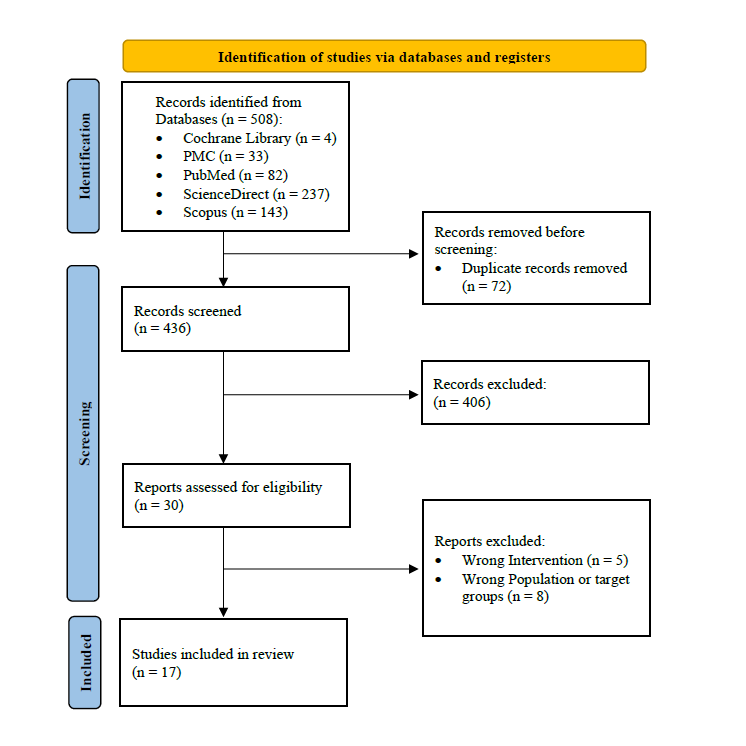
\includegraphics[width=0.95\linewidth]{figures/Prisma_flow_smartdoc_v1.png}
    \caption{Prisma Flow Diagram}
    \label{fig:1}
\end{figure*}

%%%% Another chapter to force two pages in the index
%%%%
\subsection{Publication Categorization}

This scoping review categorized studies on AI-powered virtual patients (VPs) in medical education into aforementioned four key theme.

A Venn Diagram was developed to effectively visualizes the multidimensional nature of the reviewed literature by using a color gradient to represent scoring across four themes \textit{(Figure. 2)}. This allows for quick identification of research focus overlaps, and facilitates comparative analysis of thematic relevance across individual papers and clusters of studies.

\begin{figure*}[ht]  % Use figure* instead of figure
    \centering
    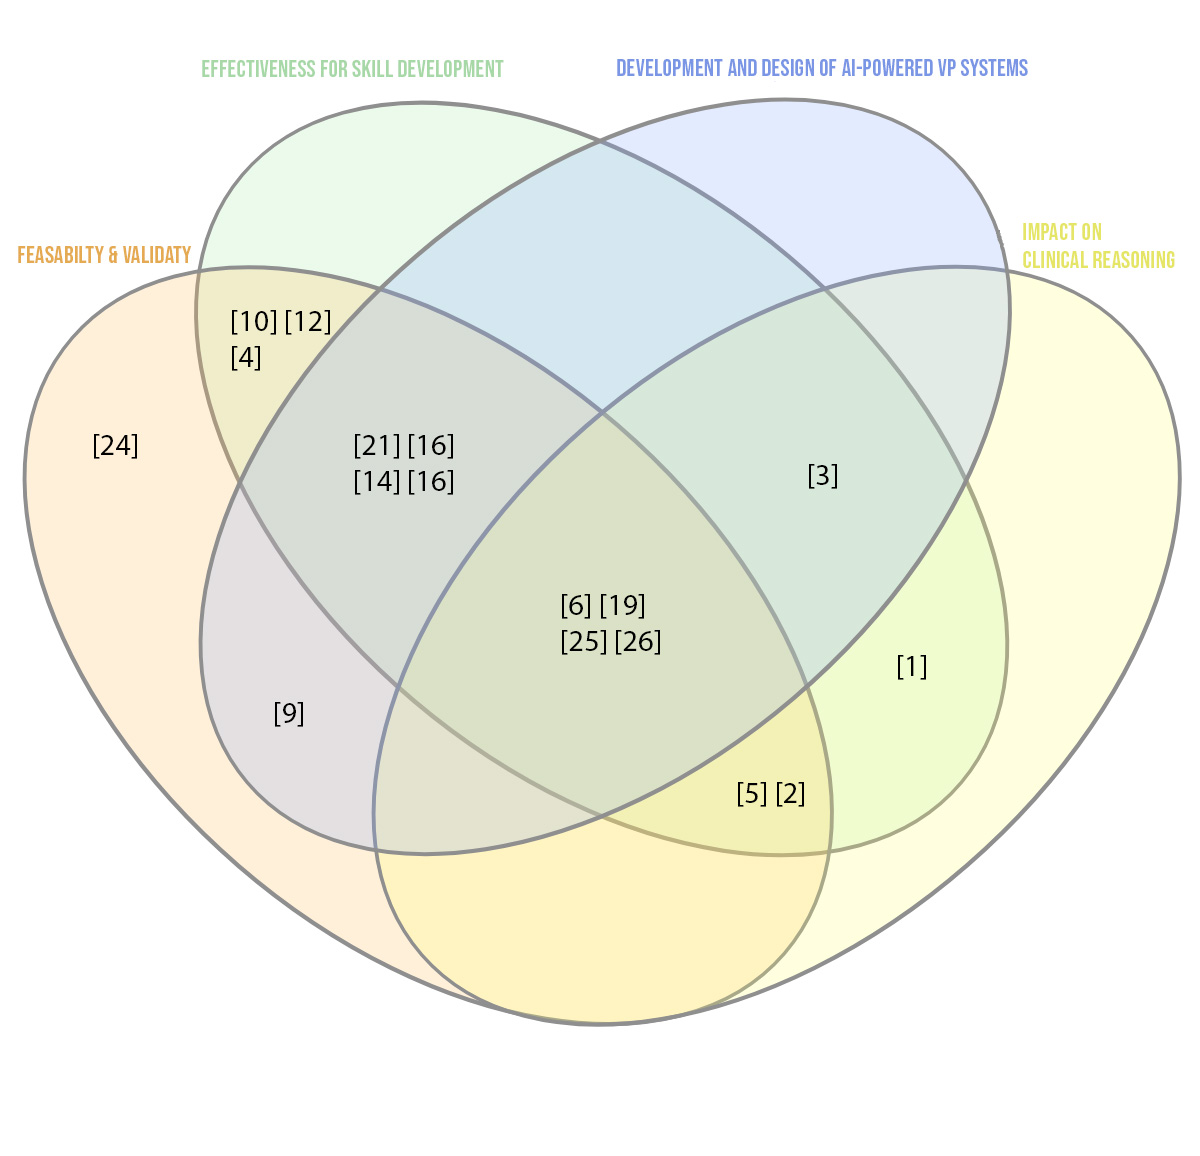
\includegraphics[width=1\linewidth]{figures/Venn.jpg}
    \caption{Venn Diagram Mapping}
    \label{fig:2}
\end{figure*} % Close the figure* environment

\subsection{Study Design}

To systematically classify the study designs, this review adopts the categorization proposed by \textit{Hanna von Gerich et al. (2022)}\cite{von2022}, which groups research articles based on their primary aim. This framework includes developing new AI technologies, improving the accuracy or efficiency of existing AI technologies, testing different algorithms or AI systems, and assessing, evaluating, or validating existing AI technologies.

\textit{Hanna von Gerich et al. (2022)} \cite{von2022} utilized this categorization to analyze the progression of AI technology in nursing, revealing a predominance of studies in the early development phases. Applying this framework in the context of AI-powered virtual patients allows for a structured analysis of the research landscape, highlighting the primary aims of included studies and enabling comparisons within the field.  Table II summarizes key study characteristics, including design and primary research aim, ensuring a structured and comparative analysis of the included studies.


\begin{table*}[h]
    \centering
    \caption{Study Design}
    \renewcommand{\arraystretch}{2}
    \begin{tabular}{@{}p{3cm}p{8cm}p{2.5cm}@{}}
        \toprule
        \textbf{Characteristic}
        & \textbf{Author, (year of publication)}
        & \textbf{Publications (n=17), n(\%)}
        \\
        \midrule
         \multicolumn{3}{@{}l}{\textbf{Study Design}} \\
        Experimental
        & \textit{Wang. (2025)} \cite{wang_application_2025}, \textit{Bruge. (2024)} \cite{brugge_large_2024}, \textit{Lippitsch. (2024)} \cite{lippitsch_development_2024}, \textit{Michael. (2022)} \cite{co_using_2022}
        & 4 (23.5\%)
        \\
        Quasi-Experimental
        & \textit{Shorey. (2019)} \cite{shorey_virtual_2019}, \textit{Anthamatten. (2024)} \cite{anthamatten_integrating_2024}, \textit{Wang. (2022)} \cite{wang_intelligent_2022}
        & 3 (17.6\%)
        \\
        Descriptive
        & \textit{Holderried. (2024)} \cite{holderried_generative_2024}, \textit{Holderried. (2024)} \cite{holderried_language_2024}, \textit{Furlan. (2021)} \cite{furlan_natural_2021}, \textit{Afzal. (2020)} \cite{s_afzal_ai_2020}, \textit{Mattei. (2024)} \cite{de_mattei_are_2024}, \textit{Wang. (2025)} \cite{wang_artificial_2025}, \textit{Maicher. (2023)} \cite{maicher_artificial_2023}, \textit{Jingrong. (2022)} \cite{jingrong_du_history-taking_2022}, \textit{Furlan. (2022)} \cite{furlan_learning_2022},\newline \textit{Maicher. (2019)} \cite{maicher_using_2019}
        &  10 (58.8\%)
        \\
        \multicolumn{3}{@{}l}{\textbf{Aim of the research}} \\
        Development of new AI \newline technologies:
        &  \textit{Furlan. (2021)} \cite{furlan_natural_2021}, \textit{Shorey. (2019)} \cite{shorey_virtual_2019},  \textit{Afzal. (2020)} \cite{s_afzal_ai_2020}, \textit{Maicher. (2023)} \cite{maicher_artificial_2023}, \textit{Wang. (2025)} \cite{wang_artificial_2025}, \textit{Lippitisch. (2024)} \cite{lippitsch_development_2024}, \textit{Wang. (2022)} \cite{wang_intelligent_2022}, \textit{Furlan. (2022)} \cite{furlan_learning_2022}.
        & 8 (47.1\%)
        \\
        Assessing, evaluating, or validating existing AI technologies:
        &  \textit{Holderried. (2024)} \cite{holderried_generative_2024}, \textit{Holderried. (2024)} \cite{holderried_language_2024}, \textit{Wang. (2025)} \cite{wang_application_2025}, \textit{Mattei. (2024)} \cite{de_mattei_are_2024}. \textit{Jingrong. (2022)} \cite{jingrong_du_history-taking_2022}, \textit{Anthamatten. (2024)} \cite{anthamatten_integrating_2024}, \textit{Brugge. (2024)} \cite{brugge_large_2024}, \textit{Michael. (2022)} \cite{co_using_2022}, \textit{Maicher. (2019)} \cite{maicher_using_2019}
        & 9 (53.9\%)
        \\
        \bottomrule
    \end{tabular}
    \label{tab:my_label}
\end{table*}


\subsection{Main findings}

The subsequent section presents a concise overview of the key findings from the included publications, organized in table format for detailed discussion. Specifically, Table II encapsulates each study's characteristics, emphasizing feasibility, effectiveness, design considerations, and the impact of AI-driven Virtual Patients (VPs) on clinical training and decision-making. Complementing this, Table III identifies factors that either facilitate or challenge technology adoption, offering a balanced perspective on the potential benefits of VPs. Collectively, these tables deliver a comparative analysis that aids in understanding the current status, practical implications, and future research directions of AI-powered VPs.

\begin{table*}[p]
    \centering
    \caption{Condensed Summary of Studies on AI-Powered Virtual Patients}
    \renewcommand{\arraystretch}{1.5}
    \setlength{\tabcolsep}{6pt} % adjust column spacing if needed
    \begin{tabular}{%
        >{\centering\arraybackslash}m{0.18\textwidth}
        >{\centering\arraybackslash}m{0.22\textwidth}
        >{\centering\arraybackslash}m{0.20\textwidth}
        >{\centering\arraybackslash}m{0.30\textwidth}}
        \toprule
        \textbf{Author (Year)} & 
        \textbf{Intervention} &
        \textbf{Population} & 
        \textbf{Key Conclusions} \\
        \midrule

        \multicolumn{4}{c}{\textbf{Feasibility and Validity}} \\
        Holderried (2024) \cite{holderried_generative_2024} & GPT-3.5 chatbot & Med/Midwifery & Realistic; useful \\
        Wang (2025) \cite{wang_application_2025} & ChatGPT SP (prompts) & Medical & Effective; cost-efficient \\
        Mattei (2024) \cite{de_mattei_are_2024} & AI-VSP cases & Healthcare & Better diagnostics; supplement \\
        Maicher (2019) \cite{maicher_using_2019} & Web VSP & Medical & Reliable; feedback support \\
        
        \midrule
        \multicolumn{4}{c}{\textbf{Skill Development}} \\
        Shorey (2019) \cite{shorey_virtual_2019} & VP comm. training & Nursing & ↑Self-efficacy; skills \\
        Jingrong (2022) \cite{jingrong_du_history-taking_2022} & WeChat VSP & Nursing & Objective; influenced by skills \\
        Michael (2022) \cite{co_using_2022} & Chatbot + tutor & Medical & Comparable to bedside \\
        Holderried (2024) \cite{holderried_language_2024} & GPT-4 chatbot & Medical & >99\% accurate; reliable \\
        Lippitsch (2024) \cite{lippitsch_development_2024} & ViPATalk avatars & Medical & Equivalent to role-play \\
        
        \midrule
        \multicolumn{4}{c}{\textbf{Development and Design}} \\
        Furlan (2021) \cite{furlan_natural_2021} & Hepius NLP/ITS & Medical & ↑Test scores; reasoning \\
        Wang (2025) \cite{wang_artificial_2025} & XueYiKu app & Students, doctors & Active learning; feedback \\
        Maicher (2023) \cite{maicher_artificial_2023} & AI VSP (ASR, RNN) & Medical & ~90\% accuracy; human-like \\
        Wang (2022) \cite{wang_intelligent_2022} & AIteach & Medical & ↑Clinical thinking \\
        Afzal (2020) \cite{s_afzal_ai_2020} & Dengue tutor bot & Medical & High usability; engagement \\
        
        \midrule
        \multicolumn{4}{c}{\textbf{Clinical Reasoning}} \\
        Furlan (2022) \cite{furlan_learning_2022} & VP NLP/ITS cases & Nurse practitioners & Consistent metrics; weak exam link \\
        Brugge (2024) \cite{brugge_large_2024} & ChatGPT feedback & Medical & Better decision-making \\
        Anthamatten (2024) \cite{anthamatten_integrating_2024} & VR + AI sims & Medical & Effective; screen > VR \\
        \bottomrule
    \end{tabular}
    \label{tab:summary-condensed}
\end{table*}

\begin{table*}[htbp]
   \centering
   \caption{Supporting and Hindering Factors for AI Adoption in Medical Education}
   \renewcommand{\arraystretch}{1.25}         % saner row height
   \setlength{\tabcolsep}{4pt}                % a bit more column padding
   \begin{tabular}{%
       >{\centering\arraybackslash}m{0.22\textwidth}%
       >{\raggedright\arraybackslash}m{0.38\textwidth}%
       >{\raggedright\arraybackslash}m{0.38\textwidth}%
   }
       \toprule
       \textbf{Factor Category} & \textbf{Supporting Factors} & \textbf{Hindering Factors} \\
       \midrule

       \textbf{Educational Potential} &
       \begin{itemize}[leftmargin=*, topsep=2pt, itemsep=2pt, parsep=0pt]
           \item Innovative, accessible learning \cite{holderried_generative_2024,de_mattei_are_2024}
           \item Overcomes traditional training limitations \cite{holderried_generative_2024}
           \item Cost-effective \cite{holderried_generative_2024,brugge_large_2024}
           \item High-quality feedback \cite{holderried_language_2024}
           \item Realistic simulations \cite{holderried_language_2024}
           \item Enhances learning through practice \cite{holderried_language_2024}
       \end{itemize}
       &
       \begin{itemize}[leftmargin=*, topsep=2pt, itemsep=2pt, parsep=0pt]
           \item Concerns about accuracy \cite{maicher_using_2019,furlan_natural_2021,s_afzal_ai_2020,brugge_large_2024}
           \item Limitations in subjective judgment and feedback mechanisms \cite{wang_application_2025,lippitsch_development_2024}
           \item Reliance on AI instead of learning \cite{holderried_language_2024}
           \item Unexpected AI behaviors \cite{holderried_language_2024}
       \end{itemize}
       \\

       \textbf{Technology \&\newline Implementation} &
       \begin{itemize}[leftmargin=*, topsep=2pt, itemsep=2pt, parsep=0pt]
           \item Technological advances in AI and NLP \cite{furlan_natural_2021,maicher_artificial_2023,wang_intelligent_2022}
           \item Improved system accuracy with training data \cite{maicher_artificial_2023}
           \item Consistent answers \cite{co_using_2022}
           \item Distance learning capabilities \cite{co_using_2022,furlan_natural_2021,wang_intelligent_2022}
       \end{itemize}
       &
       \begin{itemize}[leftmargin=*, topsep=2pt, itemsep=2pt, parsep=0pt]
           \item Technical issues \cite{shorey_virtual_2019,anthamatten_integrating_2024,de_mattei_are_2024}
           \item High implementation costs \cite{de_mattei_are_2024}
           \item Reliance on third-party services \cite{lippitsch_development_2024}
           \item Limited case variety \cite{wang_artificial_2025}
           \item Lack of system integration \cite{wang_artificial_2025}
           \item Difficulty in communication with AI \cite{anthamatten_integrating_2024}
       \end{itemize}
       \\

       \textbf{Realism \& Human Interaction} &
       \begin{itemize}[leftmargin=*, topsep=2pt, itemsep=2pt, parsep=0pt]
           \item Simulates standardized patients effectively \cite{wang_application_2025}
           \item Bridges theoretical and clinical practice \cite{de_mattei_are_2024}
       \end{itemize}
       &
       \begin{itemize}[leftmargin=*, topsep=2pt, itemsep=2pt, parsep=0pt]
           \item Lack of realism in avatars \cite{de_mattei_are_2024}
           \item Inability to fully replace human interaction \cite{de_mattei_are_2024}
           \item Absence of non-verbal cues \cite{brugge_large_2024}
       \end{itemize}
       \\

       \textbf{Cost \& Accessibility} &
       \begin{itemize}[leftmargin=*, topsep=2pt, itemsep=2pt, parsep=0pt]
           \item Cost reduction \cite{maicher_using_2019}
           \item Increased accessibility \cite{brugge_large_2024}
           \item Resource sharing \cite{wang_artificial_2025}
       \end{itemize}
       &
       \begin{itemize}[leftmargin=*, topsep=2pt, itemsep=2pt, parsep=0pt]
           \item Resource-intensive programs \cite{maicher_artificial_2023}
       \end{itemize}
       \\

       \textbf{Other} &
       \begin{itemize}[leftmargin=*, topsep=2pt, itemsep=2pt, parsep=0pt]
           \item Need for safe practice environment \cite{de_mattei_are_2024}
           \item Potential for AI improvement \cite{de_mattei_are_2024}
           \item Positive student feedback \cite{maicher_artificial_2023}
       \end{itemize}
       &
       \begin{itemize}[leftmargin=*, topsep=2pt, itemsep=2pt, parsep=0pt]
           \item Negative student attitudes towards AI feedback \cite{holderried_language_2024}
           \item Potential disengagement \cite{s_afzal_ai_2020}
           \item Preference for screen-based format over immersive VR \cite{anthamatten_integrating_2024}
       \end{itemize}
       \\
       \bottomrule
   \end{tabular}
   \label{tab:factors}
\end{table*}


\section*{\textbf{Discussion}}

This section begins with a bullet-point summary of the key findings across the four identified themes, followed by a detailed discussion of these findings.

\subsection*{\textbf{Key Findings}}

\begin{itemize}
\item \textbf{Feasibility and Validity:} AI-powered virtual patients (VSPs) are feasible and valid for medical education, showing high accuracy and realism \cite{holderried_generative_2024, wang_application_2025, maicher_using_2019, de_mattei_are_2024}. However, continuous refinement is needed to optimize accuracy and address context-dependent variability in realism.
\item \textbf{Effectiveness for Skill Development:} AI-VPs effectively enhance foundational skills, particularly history-taking, offering scalable, feedback-rich learning comparable to traditional methods \cite{holderried_language_2024, lippitsch_development_2024, shorey_virtual_2019, jingrong_du_history-taking_2022, co_using_2022}. Further research is needed to assess their impact on advanced communication skills, empathy, and long-term skill retention.
\item \textbf{Development and Design:} AI-VP systems leverage advanced technologies like NLP and ITS for realism, scalability, and pedagogical soundness \cite{furlan_natural_2021, maicher_artificial_2023, wang_artificial_2025, wang_intelligent_2022}. The use of real medical records and hybrid AI designs further enhances authenticity and sophistication.
\item \textbf{Impact on Clinical Reasoning and Decision-Making:} AI-VPs show promise in enhancing clinical reasoning and decision-making (CDM) skills, with AI feedback significantly improving CDM scores \cite{brugge_large_2024, furlan_learning_2022, anthamatten_integrating_2024}. However, further research is needed to fully quantify their long-term impact on cognitive skills.
\item \textbf{Balance between AI Innovation and Evaluation:} The field demonstrates a balance between rapid AI innovation and rigorous evaluation, with a growing body of experimental research validating AI-VPs' educational effectiveness \cite{holderried_language_2024, brugge_large_2024}.
\item \textbf{Implications for Clinical Training:} AI-VPs have transformative potential for medical education, offering scalable and effective training for foundational skills, personalized feedback, and data-driven insights \cite{co_using_2022, furlan_learning_2022}. However, strategic integration and ongoing evaluation are crucial to address limitations and maximize their pedagogical impact.
\end{itemize}

\subsubsection*{\textbf{Feasibility and Validity of AI-Powered Virtual Patients}}

AI-powered virtual patients (VSPs) demonstrate strong feasibility and validity, although optimizing accuracy and realism remains a challenge. \textit{Holderried et al. (2024)} established GPT-3.5's feasibility for patient simulation, with 94.4\% answer alignment to illness scripts and 97.9\% plausibility ratings, indicating educational acceptability and good user experience (CUQ \textit{(tool measures UX and usability of chatbots)} score: 77/100) \cite{holderried_generative_2024}. However, rare implausible answers (2.1\%) highlighted the need for refined model constraints to improve output accuracy and reduce socially desirable responses \cite{holderried_generative_2024}.

\textit{Wang et al. (2025)} reinforced AI-VP validity, showing prompt engineering significantly enhanced ChatGPT’s clinical accuracy. Iterative prompt design decreased scoring discrepancies from 29.83\% to 6.06\%, achieving 89.3\% question categorization accuracy, emphasizing iterative prompt design for valid assessments \cite{wang_application_2025}. Similarly, \textit{Maicher et al. (2019)} validated AI assessment of history-taking skills, showing computer-generated scores (87\% accuracy) closely mirrored human rater scores (90\%), with high inter-rater reliability (Intraclass correlation coefficient (ICC) \>0.75 for 81\% of categories) confirming system consistency, although complex domains require further refinement \cite{maicher_using_2019}.

\textit{De Mattei et al. (2024)} further evidenced AI-VP feasibility, with 50–87\% of students across disciplines rating them as realistic. Supporting their utility, 72–90\% reported improved diagnostic confidence. However, variable realism ratings (e.g., 16\% among physician assistant students) indicated context-dependent feasibility \cite{de_mattei_are_2024}.

\subsubsection*{\textbf{Effectiveness of AI-Powered VPs for Skill Development}}

AI-powered VPs show promise in effectively enhancing specific skills, particularly foundational skills, although nuances exist. \textit{Holderried et al. (2024)} directly addressed AI-VP effectiveness, showing GPT-4 provided structured feedback on history-taking, aligning with human raters and supporting skill improvement. \textit{Lippitsch et al. (2024)} further indicated ViPATalk's effectiveness, demonstrating equivalence to role-play for history-taking completeness while offering automated feedback and self-study benefits. This suggests AI-VPs offer a scalable alternative for foundational skill practice \cite{holderried_language_2024, lippitsch_development_2024}.

\textit{Shorey et al. (2019)} highlighted AI-VPs' potential to enhance broader communication skills, noting improved student self-efficacy and engagement, though primarily based on perceived improvements. \textit{Du et al. (2022)} indirectly supported effectiveness by validating AI-VPs' ability to provide objective history-taking skill assessments, crucial for targeted feedback. Finally, \textit{Co et al. (2022)}'s case-control study directly compared AI-VP training to traditional bedside teaching, finding comparable student performance for history-taking, suggesting AI-VPs can be as effective as real-patient interactions for foundational skills training \cite{shorey_virtual_2019, jingrong_du_history-taking_2022, co_using_2022}.

However, while AI-VPs are effective for foundational skills and feedback delivery, studies indicate limitations. \textit{Lippitsch et al. (2024)} found equivalence, not superiority, to role-play \cite{lippitsch_development_2024}. \textit{Shorey et al. (2019)} focused on perceived self-efficacy \cite{shorey_virtual_2019}, and \textit{Du et al. (2022)} primarily on assessment validity \cite{jingrong_du_history-taking_2022}. Further research is needed to assess effectiveness for advanced communication skills, empathy, and long-term skill retention.  Nevertheless, evidence indicates AI-VPs are effective tools for foundational skill development in medical education, offering scalable, accessible, feedback-rich learning.

\subsubsection*{\textbf{Development and Design of AI-Powered Virtual Patient Systems}}

AI-VP system development consistently leverages advanced technologies for realism, scalability, and pedagogical soundness. \textit{Furlan et al. (2021)} emphasized NLP integration in Hepius for realistic interaction and ITS for personalized feedback. \textit{Maicher et al. (2023)} detailed a hybrid AI system combining rule-based and neural network NLU for improved conversational fidelity. \textit{Wang et al. (2022 \& 2025)} highlighted NLP's crucial role in processing real medical records for authentic case content in AIteach and XueYiKu \cite{furlan_natural_2021, maicher_artificial_2023, wang_artificial_2025, wang_intelligent_2022}.

Beyond NLP, Intelligent Tutoring Systems (ITS) are increasingly integrated for pedagogical enhancement. \textit{Furlan et al. (2021)} incorporated an ITS module in \textit{Hepius} for step-by-step feedback. \textit{Wang et al. (2025)} implemented multidimensional automatic evaluation in XueYiKu, using radar charts for visualized feedback.  The use of real medical records, as seen in AIteach and XueYiKu \cite{wang_intelligent_2022, wang_artificial_2025}, and hybrid AI designs \cite{maicher_artificial_2023} further underscores the trend towards sophisticated, data-driven, and pedagogically informed AI-VP systems. Mobile accessibility and scalable architectures are also key design considerations \cite{s_afzal_ai_2020, wang_artificial_2025}.


\subsubsection*{\textbf{Impact of AI-Powered Virtual Patients on Clinical Reasoning and Decision-Making}}

AI-powered VPs demonstrate a promising, nuanced impact on cognitive skills, particularly clinical reasoning and decision-making. \textit{Brügge et al. (2024)} provides direct evidence of enhanced CDM with AI feedback. Their RCT showed significant CDM score improvements in students receiving AI feedback, especially in "creating context" and "securing information" subdomains \cite{brugge_large_2024}. \textit{Furlan et al. (2022)} further developed learning analytics metrics to assess specific CDM components within AI-VP simulations, offering granular performance insights \cite{furlan_learning_2022}.

\textit{Anthamatten \& Holt (2024)}'s qualitative findings align, with NP students reporting VR-AI simulations as most impactful on decision-making abilities and responsiveness to clinical changes. Students also reported increased diagnostic confidence and perceived AI-VPs as useful for history-taking and differential diagnosis development \cite{anthamatten_integrating_2024}.

However, limitations exist. \textit{Furlan et al. (2022)} found limited correlation with external hematology exam scores, suggesting VPs and traditional exams assess different competencies \cite{furlan_learning_2022}. \textit{Anthamatten \& Holt (2024)} primarily relied on student perceptions, requiring further objective validation. Despite these nuances, evidence suggests AI-VPs can positively impact cognitive skills, particularly CDM, though further research is needed to fully quantify long-term impact. \cite{anthamatten_integrating_2024}

\subsection*{\textbf{Balance between AI innovation and evaluation}}

Reflecting on methodological approaches employed across reviewed studies, a notable trend emerges concerning balance between AI innovation and rigorous evaluation. A significant portion of literature, particularly within 'Development and Design' theme, is descriptive, detailing innovative architectures, functionalities, technological advancements of AI-VP systems, showcasing rapid AI innovation in medical education. However, alongside descriptive accounts, a growing body of experimental research, as seen in 'Effectiveness' and 'Impact on Clinical Reasoning' themes, is dedicated to rigorously evaluating AI-VP pedagogical value and impact on student learning and cognitive skill development. This increasing experimental validation emphasis showcases a maturing field, moving beyond demonstrating technological feasibility towards establishing evidence for AI-powered virtual patients' educational effectiveness and optimal implementation in medical training.

\subsection*{\textbf{Interpretation in Context}}

The findings of this scoping review resonate with and expand upon existing reviews in AI-powered medical education. Similar to \textit{Stamer et al. (2023)'s} \cite{scoping2023} scoping review focused on communication skills training, it confirms the promising potential of AI and machine learning to enhance medical education, particularly by offering cost-effective, readily accessible training modalities. Both reviews align in identifying AI-VP feasibility and acceptability as key strengths, echoing \textit{Hindelang et al. (2024)'s} \cite{systematic2024} finding that chatbots can increase patient engagement and streamline data collection. This consensus across reviews strengthens the argument for the growing maturity and acceptance of AI-VP technology in medical education.

However, the current study also adds nuanced perspectives and extends beyond prior review scope. While \textit{Stamer et al. (2023)'s} scoping review focused on communication skills training, \textit{Hindelang et al. (2024)} and this study acknowledge technological limitations and challenges related to AI-VP interaction authenticity and natural language flow. Unlike those reviews, it delves deeper into the specific technological advancements (NLP, ITS, hybrid systems, learning analytics) employed to address these limitations, particularly within the "Development and Design" theme. Furthermore, unlike the narrower focus of \textit{Stamer et al. (2023)} on communication skills and \textit{Hindelang et al. (2024)} on history-taking chatbots, its broader scope, encompassing the impact on clinical reasoning and decision-making, provides a more holistic, integrated understanding of AI-VP pedagogical potential across a wider spectrum of cognitive skills essential for clinical practice. Notably, the consistent emphasis in this review on AI-generated feedback's crucial role in enhancing effectiveness, as highlighted in \textit{Holderried et al. (2024)} \cite{holderried_language_2024} and \textit{Brügge et al. (2024)} \cite{brugge_large_2024}, represents a key area of focus not explicitly emphasized in other scoping reviews. This highlights AI-generated feedback as a potentially critical mechanism for maximizing AI-VP pedagogical impact, as the reviewed studies demonstrate that detailed feedback provides a higher level of learning.

\subsection*{\textbf{Implications for Clinical Training}}

Building upon these findings and considering identified trends, key implications for clinical training and medical education emerge. The demonstrated feasibility, validity, and effectiveness of AI-powered VPs suggest transformative potential for curriculum design and technology adoption.

Firstly, findings strongly advocate for judicious AI-VP simulation integration into medical curricula, particularly in early clinical training stages, offering a scalable, accessible means for repeated practice in foundational skills. AI-VP training can be comparable to real-patient bedside teaching for history-taking skills, suggesting a viable, ethical alternative for novice learners \cite{co_using_2022}. For example, AI-VPs can be strategically integrated into early clinical training to provide students with repeated practice in history-taking, allowing them to develop proficiency before encountering real patients.

Secondly, emphasis on AI-generated feedback and learning analytics points towards a future of more personalized, data-driven medical education. AI-VPs' ability to provide structured, automated, potentially individualized feedback offers a mechanism to enhance learning efficiency and address individual student needs. Furthermore, learning analytics metrics enable continuous program improvement and curriculum refinement based on data-driven insights \cite{furlan_learning_2022}. This data can be used to identify areas where students struggle and to tailor instruction to meet their specific needs.

An interesting aspect of the clinical reasoning process is the presence of cognitive errors and biases. Furlan et al. (2021) highlight that the majority of diagnostic errors are caused by cognitive errors, rather than knowledge deficiency \cite{furlan_natural_2021}. Subsequently, Furlan et al. (2022) found that many students skipped crucial steps of the clinical interview, falling into the "early closure" mistake \cite{furlan_learning_2022}. This suggests that students may be susceptible to cognitive biases during the clinical reasoning process, which is an important consideration for future research and AI-VP development. AI-VPs can be designed to simulate scenarios that are likely to trigger cognitive biases, providing students with the opportunity to recognize and correct these errors in a safe environment. 

However, reviewed literature also underscores the importance of thoughtful, strategic implementation. As highlighted by Stamer et al. (2023) \cite{scoping2023} and Hindelang et al. (2024) \cite{systematic2024}, challenges related to authenticity, natural language flow, technological limitations, and ongoing refinement needs remain. Future curriculum design and technology adoption should prioritize:

\begin{itemize}
    \item   \textbf{Enhancing Realism and Authenticity:} Focus on improving AI-VP interaction realism and authenticity, particularly in nuanced communication aspects beyond factual accuracy.
    \item   \textbf{Strategic Integration of AI-VPs:} Integrate AI-VPs as a supplement, not a replacement, for traditional clinical experiences. For instance, AI-VPs can be used for initial skill development and practice, while real-world clinical experiences remain essential for developing advanced clinical judgment, empathy, and complex decision-making skills that require human-to-human interaction.
    \item   \textbf{Stronger Evaluation Methodologies:} Focus on robust evaluation methodologies, including RCTs and objective skill measures, to further validate AI-VP interventions' long-term educational impact. For example, future research could employ longitudinal studies to assess the long-term impact of AI-VP training on clinical skills and patient outcomes, or use standardized patient assessments to objectively measure the improvement in students' clinical skills after AI-VP training.
    \item   \textbf{Other Considerations:} Carefully consider ethical implications, data privacy, and user-centered design for responsible, equitable AI-VP implementation.
\end{itemize}

\subsection*{\textbf{Strengths and Limitations}}

This scoping review benefits from a solid search strategy across major databases and a detailed thematic analysis, providing a strong synthesis of current literature. However, it also has methodological limitations. Grey literature exclusion may have overlooked relevant findings. Initial single reviewer screening introduces potential bias, and the focus on peer-reviewed, open-access publications carries a risk of publication bias towards positive results. Future research should consider incorporating grey literature, implementing dual screening, and acknowledging potential biases when interpreting findings.


\subsection*{\textbf{Conclusion}}

This scoping review examined the current landscape of AI-powered virtual patients in medical education, synthesizing evidence across feasibility and validity, effectiveness for skill development, system design and impact on clinical reasoning.

The findings demonstrate the promising potential of AI-VPs as a valuable and increasingly sophisticated tool for medical training. AI-VPs offer a feasible, scalable, and engaging modality for delivering standardized, repeatable practice opportunities, particularly for foundational communication and history-taking skills. Moreover, AI-driven feedback and learning analytics integration within these systems offers pathways towards personalized, data-driven medical education with the potential to enhance clinical reasoning and decision-making abilities.

While challenges such as achieving complete realism, overcoming technological limitations and the need for further rigorous validation remain, the AI-VP development trajectory is clearly towards more authentic, user-friendly and pedagogically effective tools. To fully leverage this potential, medical educators should strategically integrate AI-VPs into curricula, focusing on supplementing traditional methods rather than replacing them. Researchers should prioritize investigating AI-VP impact on advanced clinical skills and long-term outcomes, specifically through longitudinal studies assessing skill retention beyond immediate training. Evaluating AI-VPs’ sustained impact on clinical competence in this manner would provide stronger evidence for their educational value and inform best practices for curriculum integration. Furthermore, developers should continue to focus on improving AI-VP realism and addressing current technological limitations. Furthermore, developers should focus on improving AI-VP realism and addressing current technological limitations. These efforts will maximize the unique strengths of AI-VPs, holding significant promise for transforming medical education and cultivating a more competent and future-ready healthcare workforce. It is crucial to invest in this rapidly evolving field and ensure AI-VPs' responsible and effective implementation in medical education and beyond.

\noindent Taken together, the evidence shows both the promise and the current
limitations of AI-powered virtual patients. While feasibility and usability
studies highlight their potential, questions remain regarding their role in
teaching complex reasoning skills, supporting metacognition, and addressing
cognitive biases in authentic contexts. 

To respond to these gaps, the next chapter presents the design and development
of the \textbf{SmartDoc} platform. Chapter~\ref{chap:ch4} demonstrates how the
theoretical principles outlined in Chapter~\ref{chap:ch2} and the empirical
findings reviewed here informed the system’s architecture, case design, and
educational features.